\chapter{Elettroni in un Potenziale Periodico}

Il potenziale in un cristallo possiede la stessa periodicità del reticolo di Bravais, cioè
\[
U(\mathbf{r}) = U(\mathbf{r}+\mathbf{R})\,,
\]
per ogni vettore di traslazione \(\mathbf{R}\).  
Pertanto, l'hamiltoniana del singolo elettrone è:
\begin{equation}
H\psi(\mathbf{r}) = \left[ -\frac{\hbar^2}{2m} \nabla^2 + U(\mathbf{r}) \right]\psi(\mathbf{r}) = \varepsilon\, \psi(\mathbf{r})\,.
\label{eqn:ham}
\end{equation}

\begin{figure}[H]
	\centering
	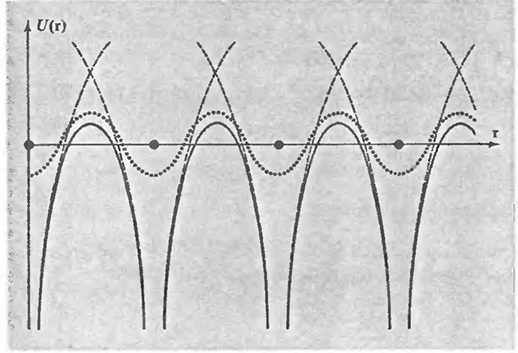
\includegraphics[width=0.5\textwidth]{images/3-Elettroni-Potenziale-Periodico/potper.png}
	\caption{Esempio di potenziale periodico in un cristallo. I punti evidenziati indicano le posizioni degli ioni.}
	\label{fig:potper}
\end{figure}

La periodicità del potenziale è la base per la \emph{teoria a bande} degli elettroni nei solidi, e conduce naturalmente all'uso della funzione d'onda di Bloch:
\[
\psi_{\mathbf{k}}(\mathbf{r}) = e^{i\mathbf{k}\cdot \mathbf{r}} u_{\mathbf{k}}(\mathbf{r})\,,
\]
con \(u_{\mathbf{k}}(\mathbf{r})\) una funzione periodica, cioè \(u_{\mathbf{k}}(\mathbf{r}) = u_{\mathbf{k}}(\mathbf{r}+\mathbf{R})\).

Questa struttura fornisce la base per l'interpretazione sperimentale delle proprietà elettroniche e ottiche dei cristalli.



\section{Teorema di Bloch}
Gli autostati dell'Hamiltoniana di singolo elettrone \ref{eqn:ham} con un potenziale con la stessa periodicità del reticolo di Bravais, sono un'onda piana moltiplicata ad una funzione con la periodicità del reticolo di Bravais
\begin{equation}
\psi_{nk}(r) = e^{i K \cdot r} u_{nk} (r), \ \ u_{nk}(r + R) = u_{nk}(r) \ \ R \in \ \text{BL}
\label{eqn:teobloch}
\end{equation}
$u_{nk}(r)$ in pratica è una funzione di r che è invariante per traslazione lungo i vettori del reticolo di Bravais. 
(\ref{eqn:teobloch}) la posso anche scrivere come:
\[\psi(r + R) = e^{i K \cdot R} \psi(r)\]
mostro che è vero:
\[ \psi(r + R) = e^{i K \cdot (r+R)} u_k(r + R) = e^{iKR}(e^{iKr} u(r)) = e^{i K R} \psi(r) \]
Notiamo anche che se questo è vero allora anche la densità di carica ha la stessa periodicità del reticolo di Bravais:
\[ \rho(r) = |\psi(r)|^2 = |\psi(r)e^{iKR}|^2 = |\psi(r + R)|^2 = \rho(r + R)  \]
all'interno del modulo ho inserito $e^{iKR}$ perché tanto il suo modulo è 1 quindi posso farlo.
\subsection{Dimostrazione del teorema di Bloch}
Per dimostrare il teorema di Bloch utilizzo la formulazione quantistica. \\\\

Definisco l'operatore traslazionale: $T_R f(r) = f(r+R)$\\
\textbf{1: Dimostro che $T_R$ commuta con H}
\[ T_R (H\psi) = H(r + R) \psi(r + R) = H(r) \psi (r+R) = H T_R \psi \implies T_R H = H T_R \]
ho che $H(r+R) = H(r)$ vale perché anche lei è periodica con il periodo del reticolo di Bravais. In ogni caso se $T_R$ ed H commutano questo significa che hanno lo stesso set di autovettori
\[ H\psi = \varepsilon \psi, \ \ T_R \psi = c(R)\psi \]
per il teorema di Bloch i loro autostati saranno:
\[ \psi(r + R) = e^{iKR}\psi(r), \ \ \psi(r + R) = c(R) \psi(r) \]
Dimostrando che queste due sono equivalenti si dimostra il teorema di Bloch. \\
Noto che 
\[ T_{R+R'}\psi(r) = T_R T_{R'} \psi(r) = T_{R'} T_{R} \psi(r) = \psi(r + R + R') \implies T_R T_{R'} =  T_{R'} T_{R} = T_{R+R'} \]
Perciò se 
\[ T_{R'}T_{R}\psi = c(R)T_{R'}\psi = c(R)c(R') \psi \ , \ T_{R'}T_{R} \psi = T_{R + R'} \psi = c(R + R')\psi \]
quindi
\begin{equation}\label{eqn:propcR}  
    c(R + R') = c(R)c(R')
\end{equation}
$T_{R}$ è un operatore unitario quindi il modulo $|c(R)|$ deve essere 1 perché è solo una traslazione e non cambia nessun altra cosa. Quindi con $R = n_1 a_1 + n_2 a_2 + n_3 a_3$ e sapendo che $T_{R} = T_{n_1 a_1 + n_2 a_2 + n_3 a_3}$ usando la proprietà \ref{eqn:propcR} ottengo:
\[ c(R) = C(a_1n_1)c(a_2n_2)c(a_3n_3) = c(a_1)^{n_1}c(a_2)^{n_2}c(a_3)^{n_3} \]
elevo alla $n_1$ perché moltiplico $n_1$ volte la stessa cosa. Se il modulo di $|c(R)|$ deve essere pari a 1 allora $c(R)$ deve essere della forma $c(R) = e^{i\mu}$ quindi in questo caso
\[ c(a_i) = e^{i2\pi x_i} \longrightarrow c(R) = e^{i2\pi(x_1n_1)}e^{i2\pi(x_2n_2)}e^{i2\pi(x_3n_3)} = e^{i 2\pi (x_1 n_1 + x_2n_2 + x_3 n_3)}   \]
sappiamo che $k = (x_1 b_1 + x_2b_2 + x_3 b_3)$ questo vuol dire che 
\[ C(R) = e^{i k \cdot R} \]
perché se $R = n_1 a_1 + n_2 a_2 + n_3 a_3$ e $K = x_1 b_1 + x_2b_2 + x_3 b_3$ allora facendo il prodotto scalare ho che $a_i \cdot b_j = 2\pi \delta_{ij}$ quindi $K \cdot R = 2\pi (x_1 n_1 + x_2n_2 + x_3 n_3)$ perciò
\[ T_R \psi = \psi (r + R) = c(R) \psi = e^{i K\cdot R} \psi (r) \]
Ed è il teorema di Bloch.

\subsection{Dimostrazione teorema di Bloch con trasformata}
Espandiamo la funzione d'onda e il potenziale come:
\[\psi(\mathbf{r})= \sum_q C_q\cdot e^{i\mathbf{q}\cdot \mathbf{r}} \hspace{0.3cm} U(\mathbf{r})= \sum_k U_k\cdot e^{i\mathbf{k}\cdot \mathbf{r}}\]
Con $\mathbf{r}$ vettore del B.L. e $\mathbf{k}$ vettore del R.L.\\\\
Dimostriamo che la trasformata del potenziale $U_k = U^*_k = U_{-k}$:
\[U_k = \int U(\mathbf{r}) \cdot e^{-i\mathbf{k}\cdot \mathbf{r}}\d\mathbf{r} \implies U^*_k = \int U^*(\mathbf{r}) \cdot e^{i\mathbf{k}\cdot \mathbf{r}}\d\mathbf{r} =  \int U(\mathbf{r}) \cdot e^{-i(-\mathbf{k})\cdot \mathbf{r}}\d\mathbf{r} = U_{-k}\]
Per $U(\mathbf{r}) = U(-\mathbf{r})$ si ottiene:
\begin{align*}
	U_k &= \int U(\mathbf{r}) \cdot e^{-i\mathbf{k}\cdot \mathbf{r}}\ \d\mathbf{r} \hspace{0.2cm}\text{invertiamo} \hspace{0.2cm} \mathbf{r} \to -\mathbf{r} \implies\\ 
	\implies U_k &= \int U(\mathbf{r}) e^{-i(\mathbf{-k})\cdot \mathbf{r}}\ \d\mathbf{r}= U_{-k} = U_k^*
\end{align*}
Ora risolviamo l'equazione agli autovalori:\\\\
\begin{enumerate}
    \item Termine cinetico :
    \[-\frac{\hbar^2\nabla^2}{2m}\cdot \psi(\mathbf{r)} =-\frac{\hbar^2\nabla^2}{2m}\cdot \sum_q C_q\cdot e^{i\mathbf{q}\cdot \mathbf{r}} = \frac{\hbar^2}{2m}\sum_q q^2 \cdot C_q\cdot \cdot e^{i\mathbf{q}\cdot \mathbf{r}}\]
    \item Termine potenziale :
    \[U(\mathbf{r}) \cdot \psi(\mathbf{r}) = \sum_{k,q} C_q U_k e^{i(\mathbf{k}+\mathbf{q})\cdot \mathbf{r}}\]
    Sostituiamo $\mathbf{q'} = \mathbf{q}+\mathbf{k}$
    \[U(\mathbf{r}) \cdot \psi(\mathbf{r}) = \sum_{k,q'} C_{q'-k} U_k e^{i\mathbf{q'\cdot r}}\]
    Usiamo il fatto che la scelta del indice è arbitraria (indice muto) ed otteniamo:
    \[U(\mathbf{r}) \cdot \psi(\mathbf{r}) = \sum_q \sum_k C_{q-k} U_k e^{i\mathbf{q\cdot r}}\]
\end{enumerate}
Da cui l'equazione diventa:
\[\frac{\hbar^2}{2m}\sum_q q^2 \cdot C_q\cdot \cdot e^{i\mathbf{q}\cdot \mathbf{r}}+ \sum_q \sum_k C_{q-k} U_k e^{i\mathbf{q\cdot r}} = \varepsilon \cdot \sum_q C_q\cdot e^{i\mathbf{q}\cdot \mathbf{r}}\]
\[\sum_q e^{i\mathbf{q}\cdot \mathbf{r}} \cdot \bigl[\biggr(\frac{\hbar^2}{2m}\cdot \mathbf{q}^2 -\varepsilon\biggr)C_q + \sum_{k} U_k C_{q-k}\bigr]= 0\]
Siccome $\{\mathbf{q}\}$ è un set di vettori orto-normali che soddisfano le Born Van-Karman Conditions, possiamo imporre a zero ciascun coefficiente ed ottenere per $\mathbf{q} = \mathbf{k}- \mathbf{K}$ e $\mathbf{k'}= \mathbf{k}+\mathbf{K}$ con $\mathbf{k}$ vettore della prima zona di brillouin e $\mathbf{K}$ vettore del R.L.
\[\biggr(\frac{\hbar^2}{2m}\cdot (\mathbf{k-K})^2 -\varepsilon\biggr)C_{k-K} + \sum_{k'} U_{k'-K} C_{k-k'}= 0\]
Abbiamo quindi un sistema di n equazioni per ogni valore di $\mathbf{k}$ permesso appartenente alla prima zona di Briollouin, da cui la funzione d'onda può essere riscritta come:
\[\psi(\mathbf{r}) = \sum_q C_q e^{i\mathbf{q}\cdot\mathbf{r}} = \sum_K C_{k-K}e^{i(\mathbf{k}-\mathbf{K})\cdot \mathbf{r}} =e^{i\mathbf{k}\cdot\mathbf{r}} \cdot  \sum_K C_{k-K}e^{-i\mathbf{K}\cdot \mathbf{r}} = e^{i\mathbf{k}\cdot\mathbf{r}} \cdot u_k(\mathbf{r}) \]
\section{Condizioni di Born-Von Karman}
Sono delle condizioni al contorno periodiche:
\[ \psi(r + N_i a_i) = \psi(r) \ , \ i = 1,2,3 \]
$N_i a_i$ è il numero di celle nel solido in ogni direzione e gli $a_i$ sono i vettori primitivi. Per il teorema di Bloch
\[ \psi_{nk}(r + N_i a_i) = e^{i N_i k \cdot a_i} \psi_{nk}(r) \]
ma abbiamo bisogno che $e^{i N_i k \cdot a_i} = 1$ per soddisfare la condizione di periodicità. Quindi se $k = x_1 b_1 + x_2b_2 + x_3 b_3$ allora ho che 
\[  e^{i N_i k \cdot a_i}  =  e^{i 2 \pi N_i x_i} = 1 \implies x_i = \frac{m_i}{N_i} \]
ed è discreto, è un intero diviso per il numero di celle in quella direzione i.\\\\ 
La forma generale del vettore d'onda quindi è:
\[ k = \sum_{i = 1}^3 \frac{m_i}{N_i}b_i \]
Questo significa che il fatto che la lunghezza di un reticolo è limitata causa la discretizzazione dei vettori k. \\\\
Quanti stati sono permessi? \\
Il volume dello spazio k per ogni k permesso è dato da, dato $k =  \frac{m_1}{N_1}b_1 + \frac{m_2}{N_2}b_2 + \frac{m_3}{N_3} b_3$ (ricordando che N è il numero di celle in quella direzione): 
\[ \Delta k = \frac{b_1}{N_1} \cdot \left( \frac{b_2}{N_2} \times \frac{b_3}{N_3} \right) = \frac{1}{N} b_1 \cdot (b_2 \times b_3) \]
quindi $b_1 \cdot (b_2 \times b_3)$ è il volume di un solido costituito da 3 vettori non collineari quindi è il volume della cella primitiva del reticolo reciproco. \\
Il numero di vettori d'onda permessi in una cella primitiva del reticolo reciproco è uguale al numero di siti nel cristallo, $\rho$ è la densità di sttai nel k-space
\[ \Delta k = \frac{(2\pi)^3}{a^3 } = \frac{(2\pi)^3}{V} \hspace{2cm} \rho = \frac{V}{(2\pi)^3} \]
\subsubsection{commenti sul teorema di Bloch}
1) $\psi_{nk}$ \textbf{non è un autostato del momento} $\vec{p} = (\frac{\hbar}{i})\vec{\nabla}$ 
\begin{equation*}
\frac{\hbar}{i} \vec{\nabla} \psi_{nk} = \frac{\hbar}{i} \vec{\nabla}(e^{i k \cdot r} u_{nk}(r)) = \hbar k \psi_{nk} + e^{i k\cdot r} \frac{\hbar}{i} \vec{\nabla} u_{nk}(r)
\end{equation*}
Dovremmo vedere k come un numero quantico caratteristico della simmetria traslazionale di un potenziale periodico, come il momento p che è un numero quantico caratteristico dell'intera simmetria traslazionale dello spazio libero. \\\\
2) se $k$ è confinato alla prima zona di Brillouin e $k'$ è al di fuori della prima zona di Brillouin, allora posso scrivere 
\[\mathbf{k' = k + K}\]
dove $K$ è un vettore del reticolo reciproco, infatti: 
\[ \psi(r + R) = e^{ik' \cdot R}\psi(r) = e^{i k \cdot R + iK \cdot R} \psi(r) = e^{i k \cdot R}\psi(r) \]
3) \textbf{La funzione d'onda dipende da un indice discreto $\mathbf{n}$ e da un continuo $\mathbf{k}$ appartenente alla prima zona di Brillouin}.\\\\
Data l'equazione di Schrodinger 
\[ H\psi = \left( -\frac{\hbar^2}{2m}\nabla^2 + U(r) \right) \psi = \varepsilon \psi \]
con delle funzioni d'onda di Bloch 
\[ \psi(r) = e^{i k \cdot r} u(r) \]
ottengo 
\[ H_k u_k = \left( -\frac{\hbar^2}{2m} \left( \frac{1}{i}\vec{\nabla} + k \right)^2 + U(r) \right) u_k(r) = \varepsilon_k u_k(r) \]
ricordando che $u_k(r) = u_k(r+R)$ \\
Per le condizioni periodiche al contorno, il problema è ristretto ad una sola cella del cristallo, siccome il volume è fissato ci aspettiamo per ogni valore $k$ che l'equazione di schrodinger abbia una \textbf{famiglia infinita di soluzioni con autovalori discreti di indice} $\mathbf{n}$ (come nel caso del elettrone libero in una scatola, ho livelli quantizzati).\\\\
4) \textbf{Periodicità dell'energia e indice di banda.}\\
Posso assegnare gli indici $\mathbf{n}$ ai livelli in modo tale che per un dato $\mathbf{n}$ gli autostati e gli autovalori sono funzioni periodiche in $\mathbf{k}$ del reticolo reciproco (c'è solo $\mathbf{n}$ perché nella nostra trattazione non viene considerata l'interazione con gli spin)
\[ \psi_{n,k}(r + R) = e^{i k \cdot R} \psi_{n,k}(r) \]
\[ \psi_{n, k + K}(r )= \psi_{nk}(r) \]
\[ \varepsilon_{n, k + K}(r )= \varepsilon_{nk}(r) \]
se $\psi$ è periodico nello spazio k allora lo sarà anche l'energia. $\varepsilon_n (k)$ è detta \textbf{banda di energia} ed $\mathbf{n}$ è l'indice della banda. È una banda perché se l'energià è periodica in $\mathbf{k}$ e continua avrà un limite superiore ed uno inferiore, quindi i livelli energetici sono compresi tra questi due limiti. \\\\
5) \textbf{Velocità}\\
Un elettrone in un livello specificato dall'indice di banda n e con vettore d'onda k ha una velocità data da:
\[ v_n (k) = \frac{1}{\hbar} \nabla_k \varepsilon_n (k) \]
$v_n(k)$ è la velocità di un pachetto d'onda, si nota che la velocità di un elettrone è in relazione al gradiente dell'energia questo perché è limitata, ci sono punti dove la velocità sarà 0 perché lo sarà anche il gradiente. 
\begin{figure} [H]
	\centering
	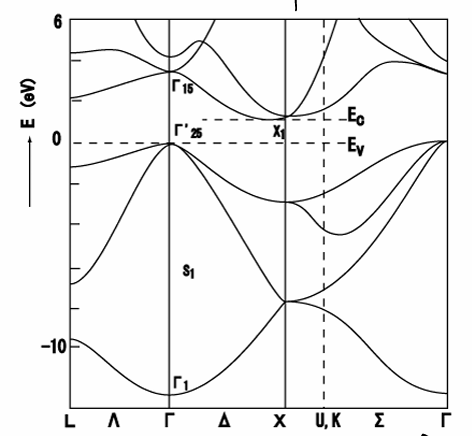
\includegraphics[width=0.5\textwidth]{images/3-Elettroni-Potenziale-Periodico/esbande.png}
	\caption{esempio di bande in un cristallo FCC. le bande vengono riempire sempre seguendo il principio di esclusione di Pauli}
	\label{fig:esbande}
\end{figure}

\subsection{Superficie di Fermi}
Siccome le bande vengono riempite sempre seguendo il principio di esclusione di Pauli un certo numero di bande può essere completamente pieno e altre invece possono rimanere vuote, la differenza di energia tra il livello occupato più alto e il livello non occupato più basso è detto \textbf{gap}. \\
Un certo numero di bande invece potrebbe essere parzialmente pieno e per ogni banda di questo tipo ci sarà una superficie nello spazio k che separa i livelli occupati da quelli non occupati. L'insieme di tutte queste superfici è noto come \textbf{superificie di Fermi}, ed è una generalizzazione degli elettroni liberi nella sfera di Fermi al modello di Bloch. \\
$\varepsilon_n(k) = \varepsilon_F$ definisce la superificie di Fermi

\subsection{Densità di stati}
Ora ho una serie di bande che contribuiscono in maniera diversa alla densità degli stati, quindi la densità di stati dipenderà da n. \\
Ciò che dovrò fare sarà calcolare una quantità che è una somma pesata  sui livelli elettronici di diverse proprietà di un singolo elettrone, e queste quantità sono del tipo:
\[ Q = 2 \sum_{n,k} Q_n (k) \]
Per ogni n la somma è su tutti i k permessi dando livelli distinti. Nel limite di un cristallo molto grande i valori permessi dei k si infittiscono diventando sempre più vicini tra di loro, quindi al posto della somma posso integrare. Dato che il volume dello spazio k per k permesso ha lo stesso valore del caso in cui l'elettrone è libero, tutto ciò che è stato ottenuto nel caso dell'elettrone libero rimane valido:
\begin{equation} q = \lim_{v \to \infty} \frac{Q}{V} = 2 \sum_n \int \frac{\d{k}}{(2\pi)^3} Q_n(k) \label{eqn:q1} \end{equation}
$Q_n (k)$ dipende da n e k solo attraverso l'energia $\varepsilon_n(k)$, qundi sempre seguendo l'analogia col caso con l'elettrone libero uno può definire la densità di stati per unità di volume per unità di volume $g(\varepsilon)$ in modo che q abbia la forma:
\begin{equation}\label{eqn:q2}
    q = \int \d{\varepsilon} g(\varepsilon)Q(\varepsilon)
\end{equation}
confrontando \ref{eqn:q1} e \ref{eqn:q2} trovo che 
\[ g(\varepsilon) = \sum_n g_n (\varepsilon) \]
con l'introduzione di questa definizione di densità di stati
\[ g_n (\varepsilon) = \int \frac{\d{k}}{4\pi^3}\delta(\varepsilon - \varepsilon_n(k)) \]
che indica il numero di stati compreso tra $\varepsilon$ ed $\varepsilon_n$. \\
Se voglio trovare anche l'energia totale
\[ U = \sum_{k,n} \varepsilon_n(R) f(T, \varepsilon_n(R)) \]
dove $\varepsilon_n(R)$ è una funzione di $Q_n(k)$ ed $f(T, \varepsilon_n(R))$ è la distribuzione di Fermi Dirac. \\
Un altro modo per rappresentare la densità di stati è riportato nelle figure \ref{fig:densst1} e \ref{fig:densst2} e si fa comportandoci come nel caso dell'elettrone libero. 
\begin{figure}[H]
	\centering
	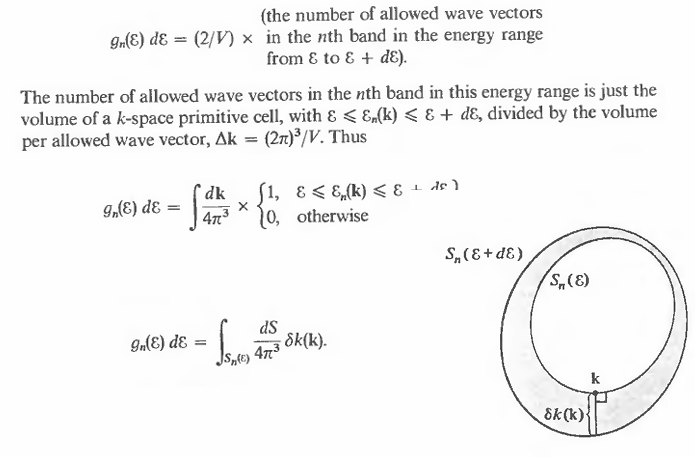
\includegraphics[width=\textwidth]{images/3-Elettroni-Potenziale-Periodico/densst1.png}
	\caption{}
	\label{fig:densst1}
\end{figure}
\begin{figure}[H]
	\centering
	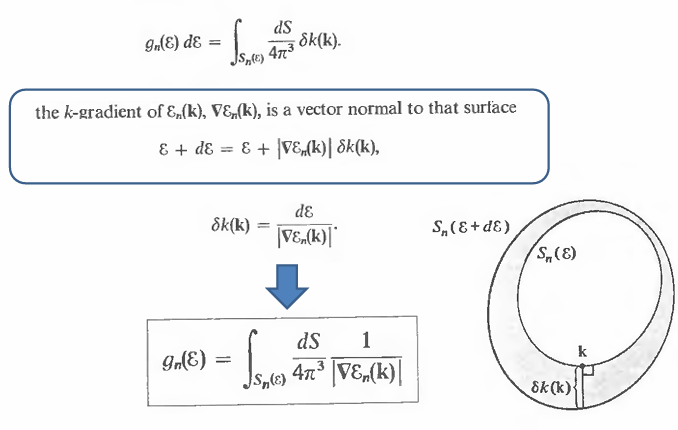
\includegraphics[width=\textwidth]{images/3-Elettroni-Potenziale-Periodico/densst2.png}
	\caption{}
	\label{fig:densst2}
\end{figure} 
